This experiment is conducted to understand two questions. One is how different variable types have impact to runtime performance.
The other is how initialization of Vec size has impact to runtime performance. 
In this experiment, we focus on owner, reference, and slice as a variable of sequence values. 
Since these variables have different memory representation, there might be differences among time for access to actual values of each variables.

To evaluate this assumption, we use the three types of complex object: CustomerOwned, CustomerBorrowed and CustomerSlice. 
At first, we generate source Vecs for all fields, Vecs which contain all elements used for corresponding fields of objects.
For example, all of i32 elements used for key field in 1 million Customer object are stored in Vec$<$i32$>$ with 1 million i32 elements. 
Later, these i32 elements are moved to be owned or borrowed by the object's fields.

Next, 1.5, 1.8, 2.5, 2.8, 3.5, and 3.8 million of Customer objects are created and stored in Vec. 
When a Customer Vec is created, whether size of Vec is initialized is controlled. 
Finally, serialization of Customer object is performed as an operation forcing program to access all of fields in the object.
This serialization is performed each Customer objects in the Vec. We measure total runtime to serialize all of Customer objects 
stored in Vec. 

\subsection{Result}
\label{sec:history}
The result is shown in Figure~\ref{fig:rustaccessinit} and Figure~\ref{fig:rustaccessnoinit}.
Figure~\ref{fig:rustaccessinit} is comparison of the runtime performance among different Customer object types with Vec size initialization.
Figure~\ref{fig:rustaccessnoinit} is comparison in the same set of experiment except Vec size is not initialized. 
The blue, yellow, and green chats represent runtime of access to fields of CustomerOwned, CustomerBorrowed, and CustomerSlice objects respectively.

No matter Vec size initialized or not, differences of runtime for accessing objects are not remarkable among different object types. 
The percent increase in runtime of accessing to fields of from 1.5 to 3.8 million CustomerOwned objects is 121\% if the Vec is initialized, 554\% if the Vec is not initialized.

Considering the differences of percent increase of runtime whether the Vec is initialized or not, 
Figure\ref{fig:init_vs_noinit} the comparison of runtime access to fields of CustomerOwned object with and without Vec Initialization.
For 3.8 million of objects, the difference of runtime to access to the objects is 38745 secounds; program without Vec initialization is 60\% slower than one with the initialization.

\begin{figure}[htb]
    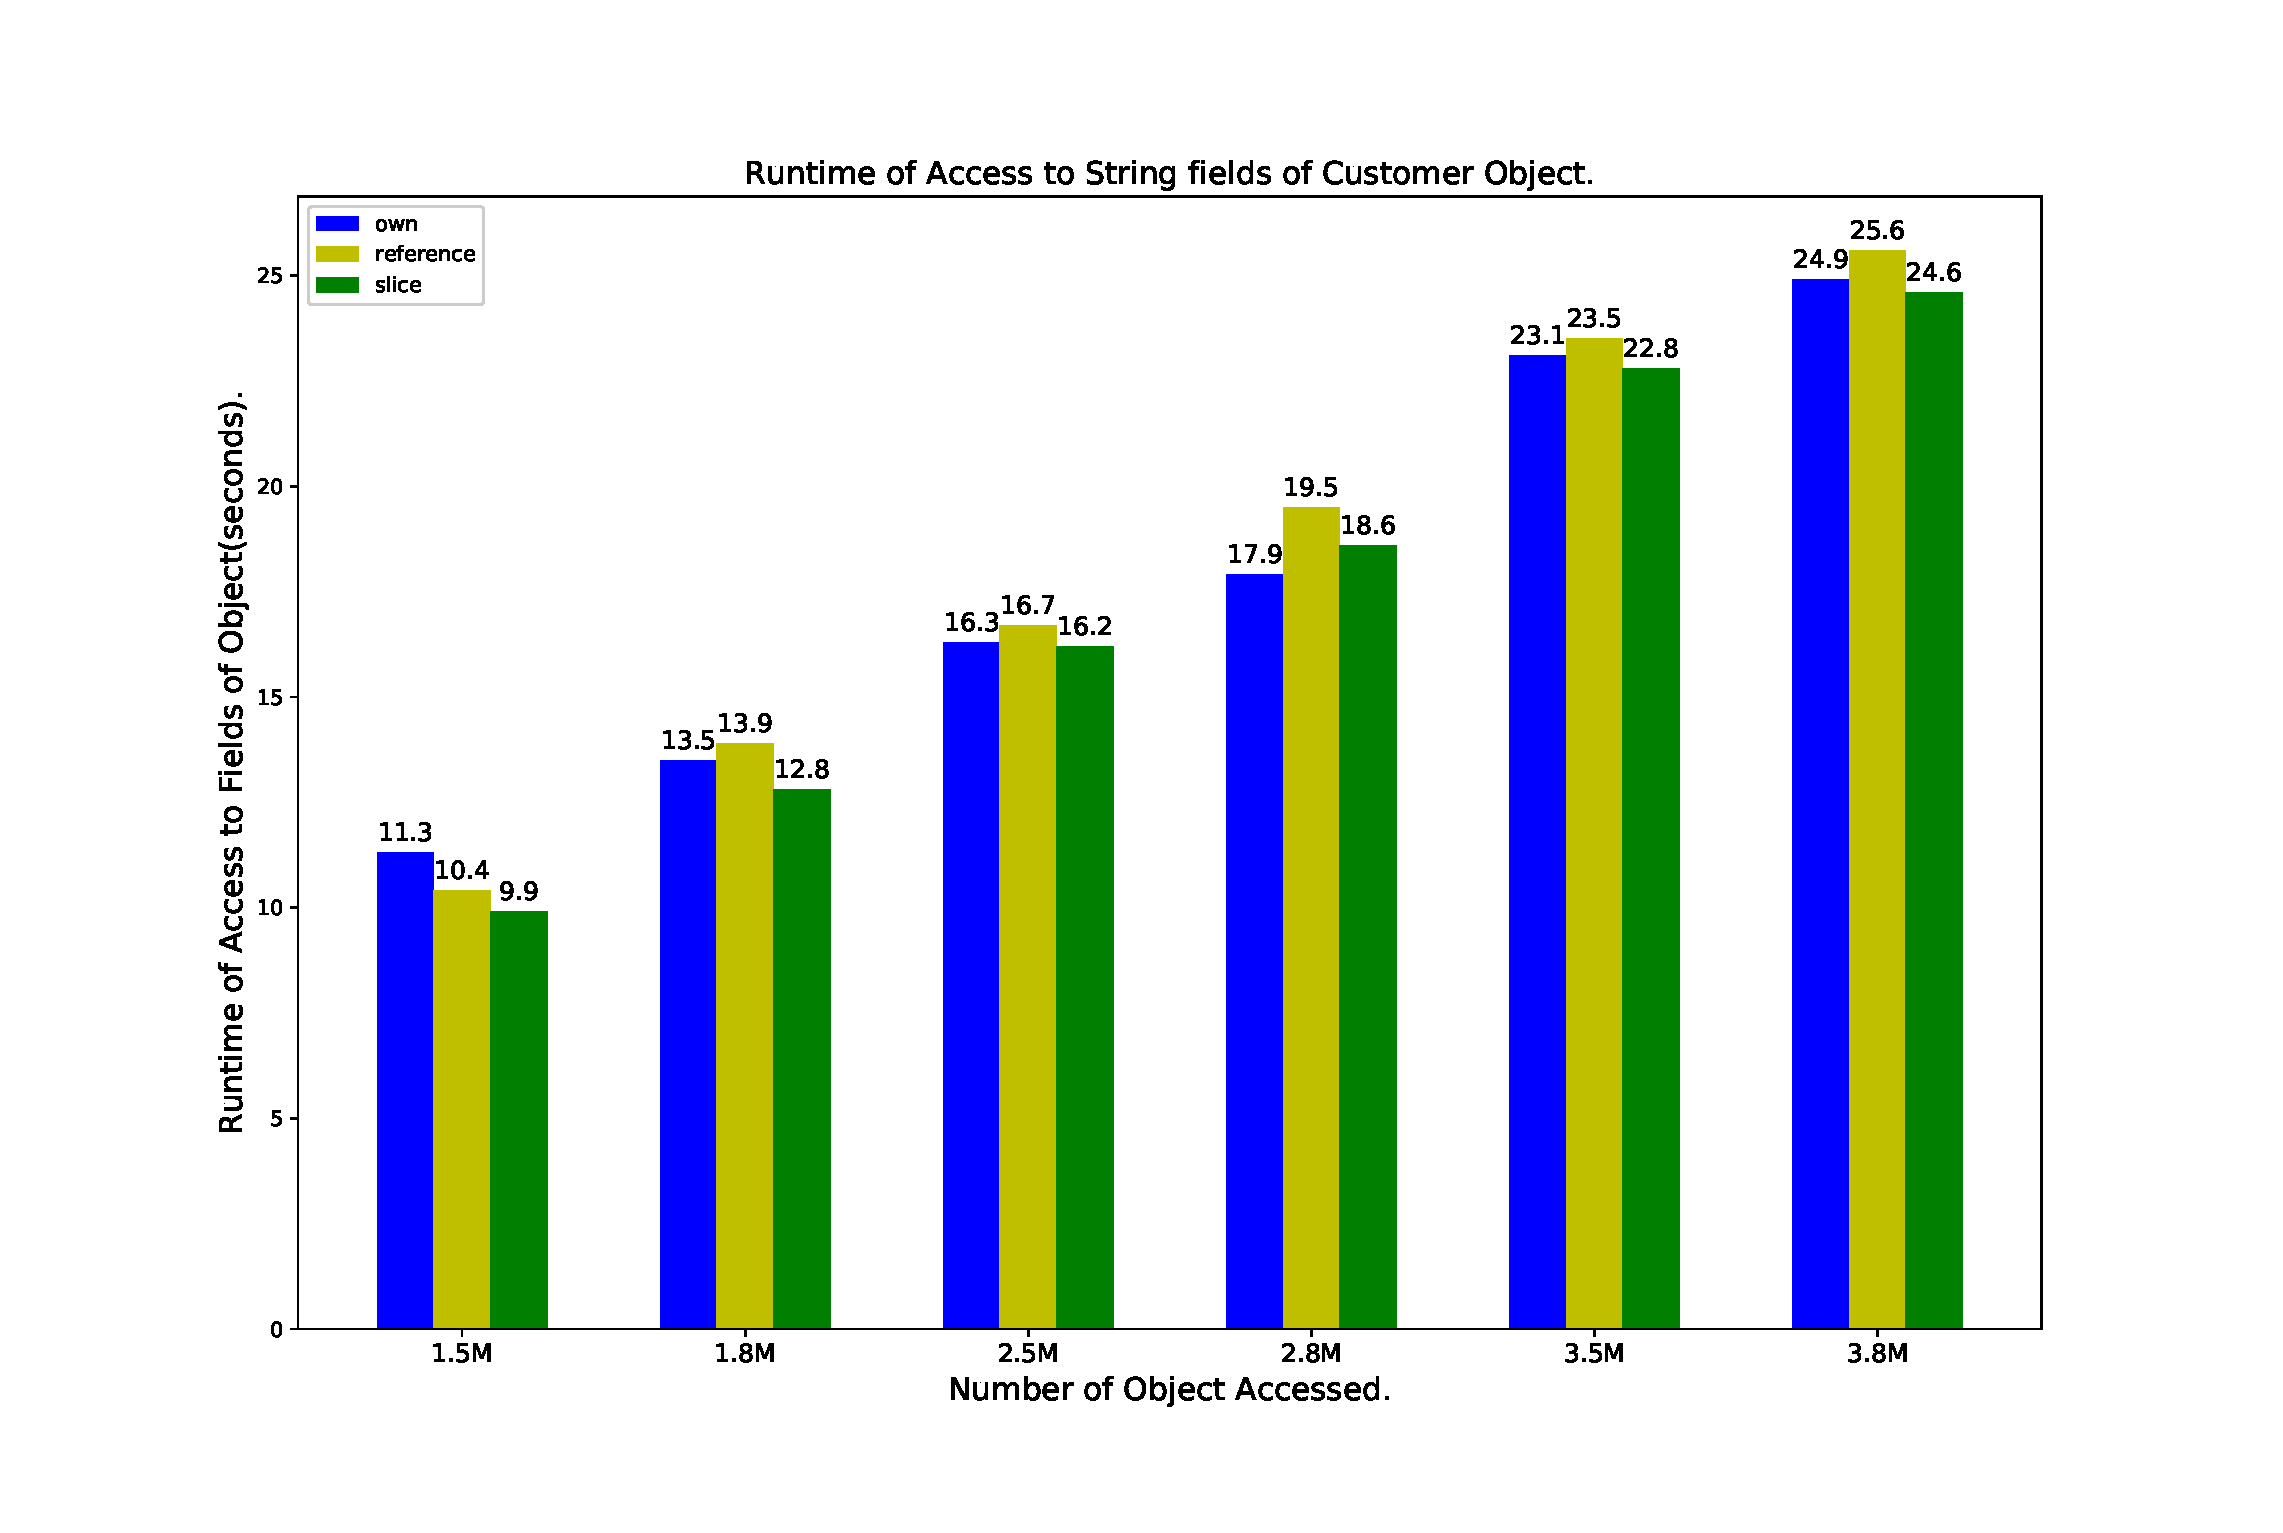
\includegraphics[width=15cm]{rust_access_different_poniter_init.eps}
    \caption{Runtime of Access to Different Pointer Types with Vec Size Initialization}
    \label{fig:rustaccessinit}
\end{figure}

\begin{figure}[htb]
    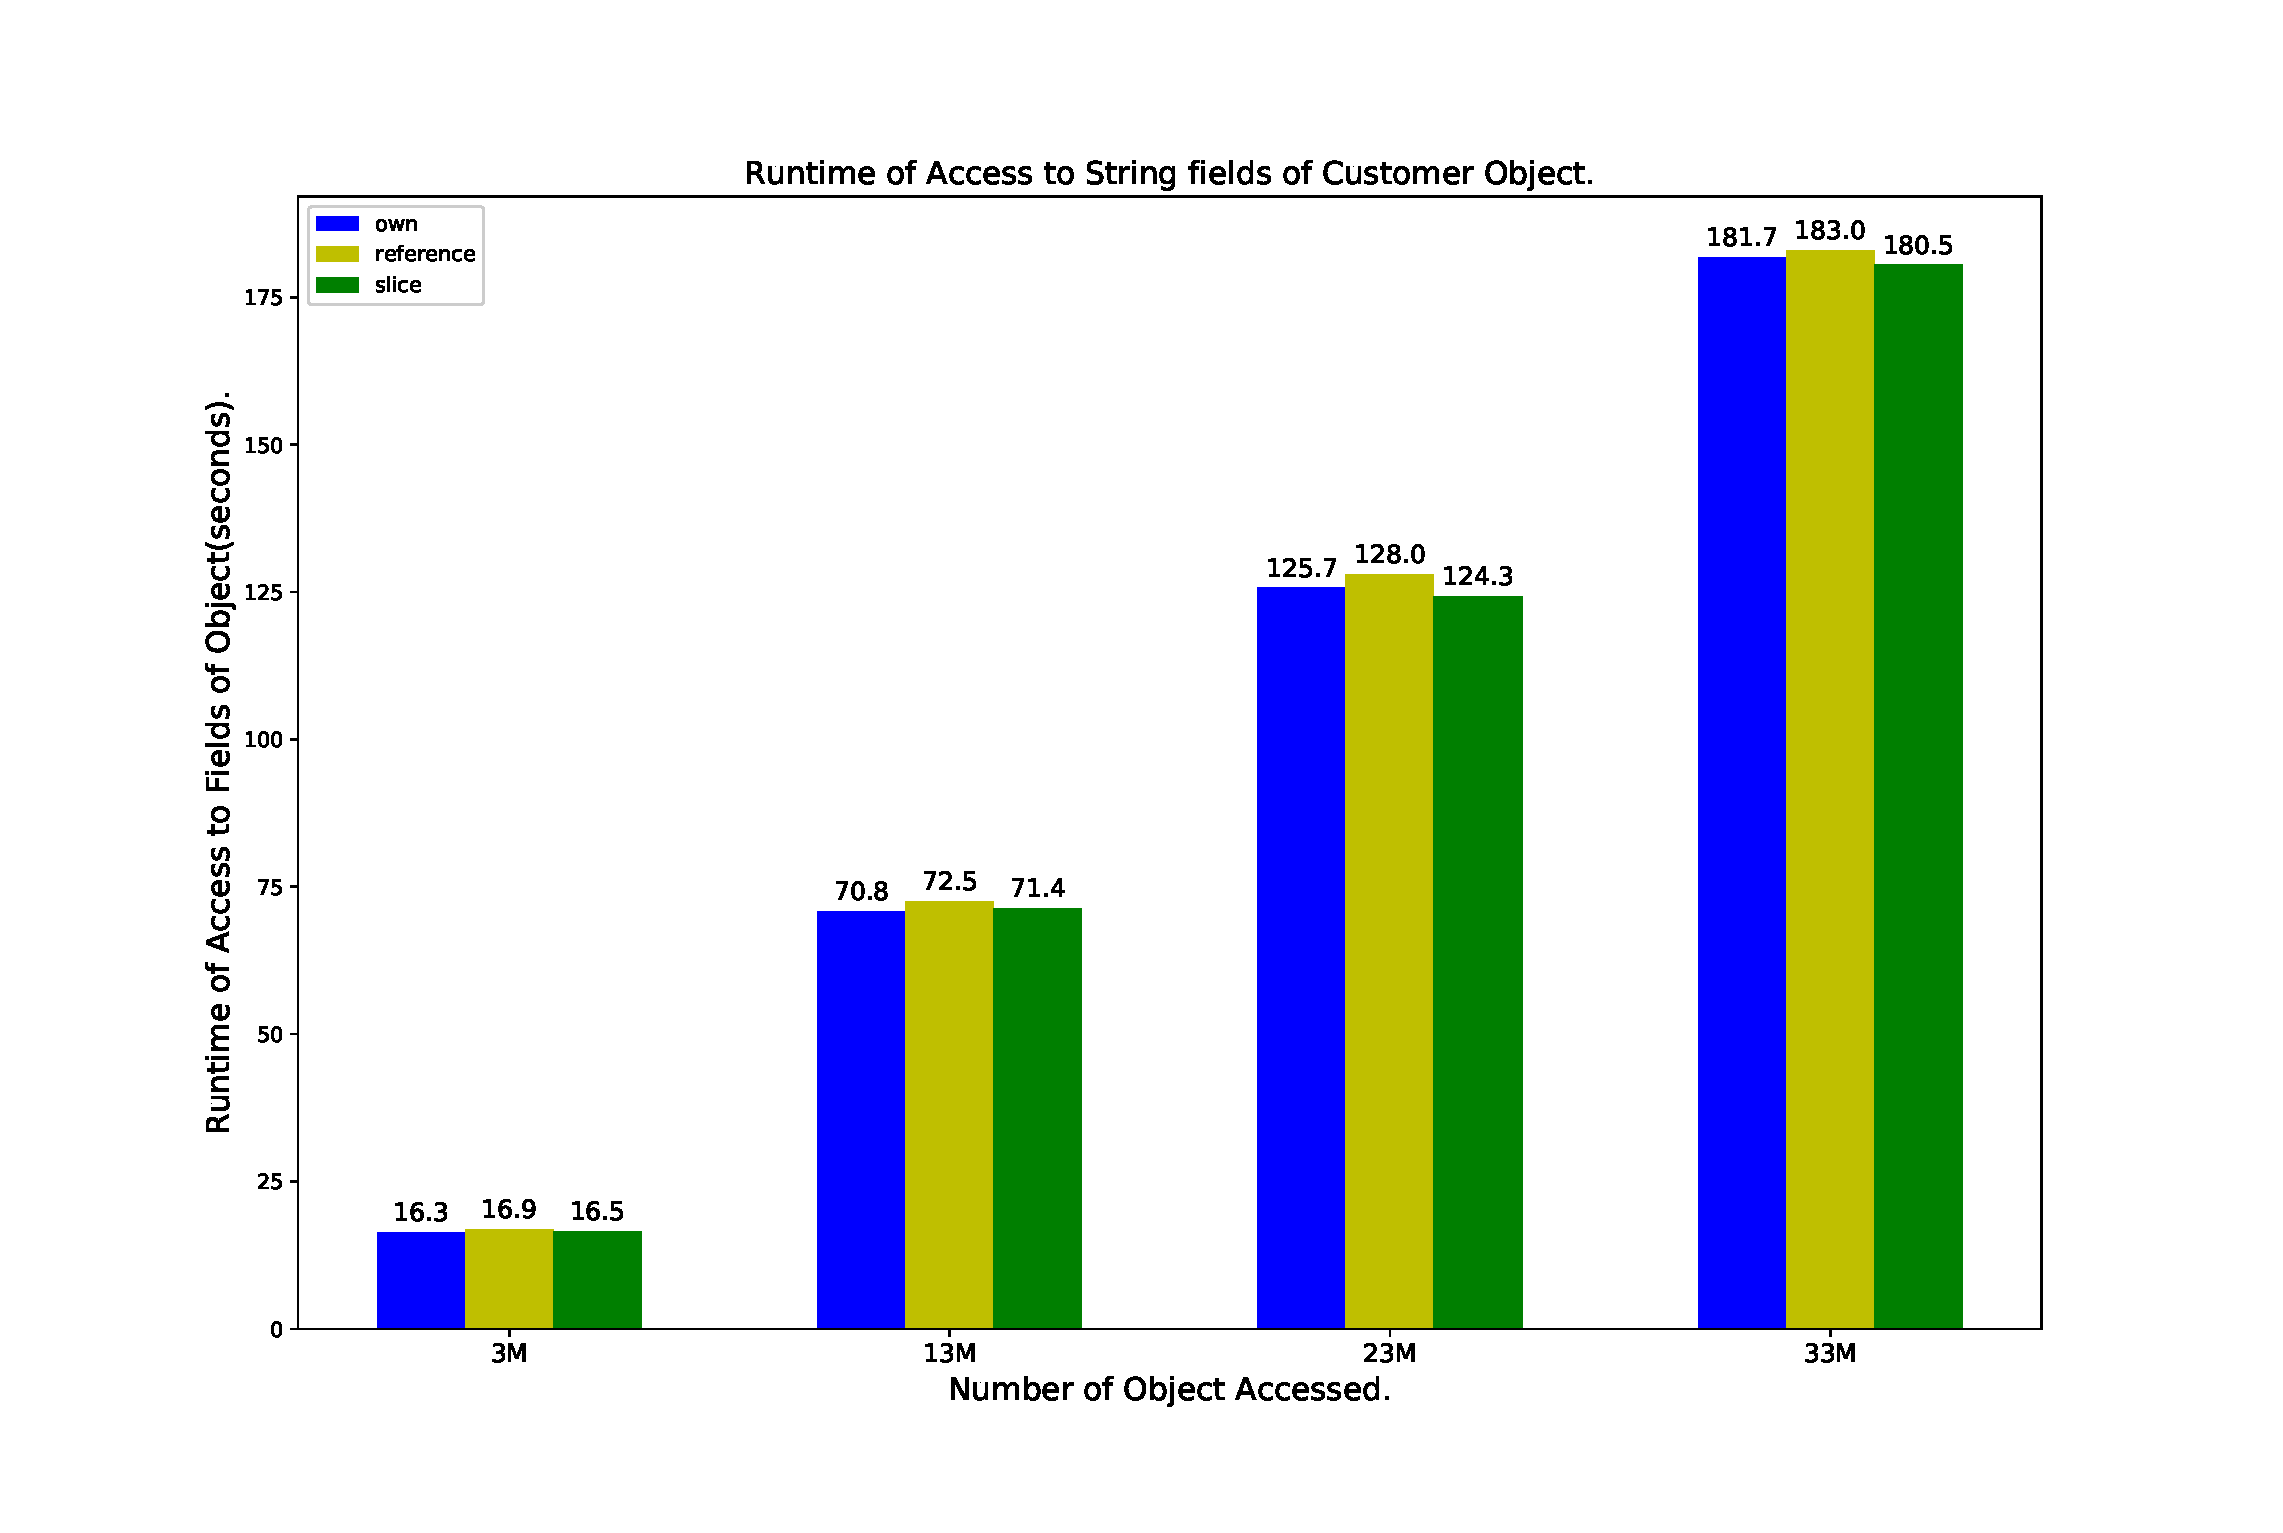
\includegraphics[width=15cm]{rust_access_different_poniter_noinit.eps}
    \caption{Runtime of Access to Different Pointer Types without Vec Size Initialization}
    \label{fig:rustaccessnoinit}
\end{figure}

\begin{figure}[htb]
    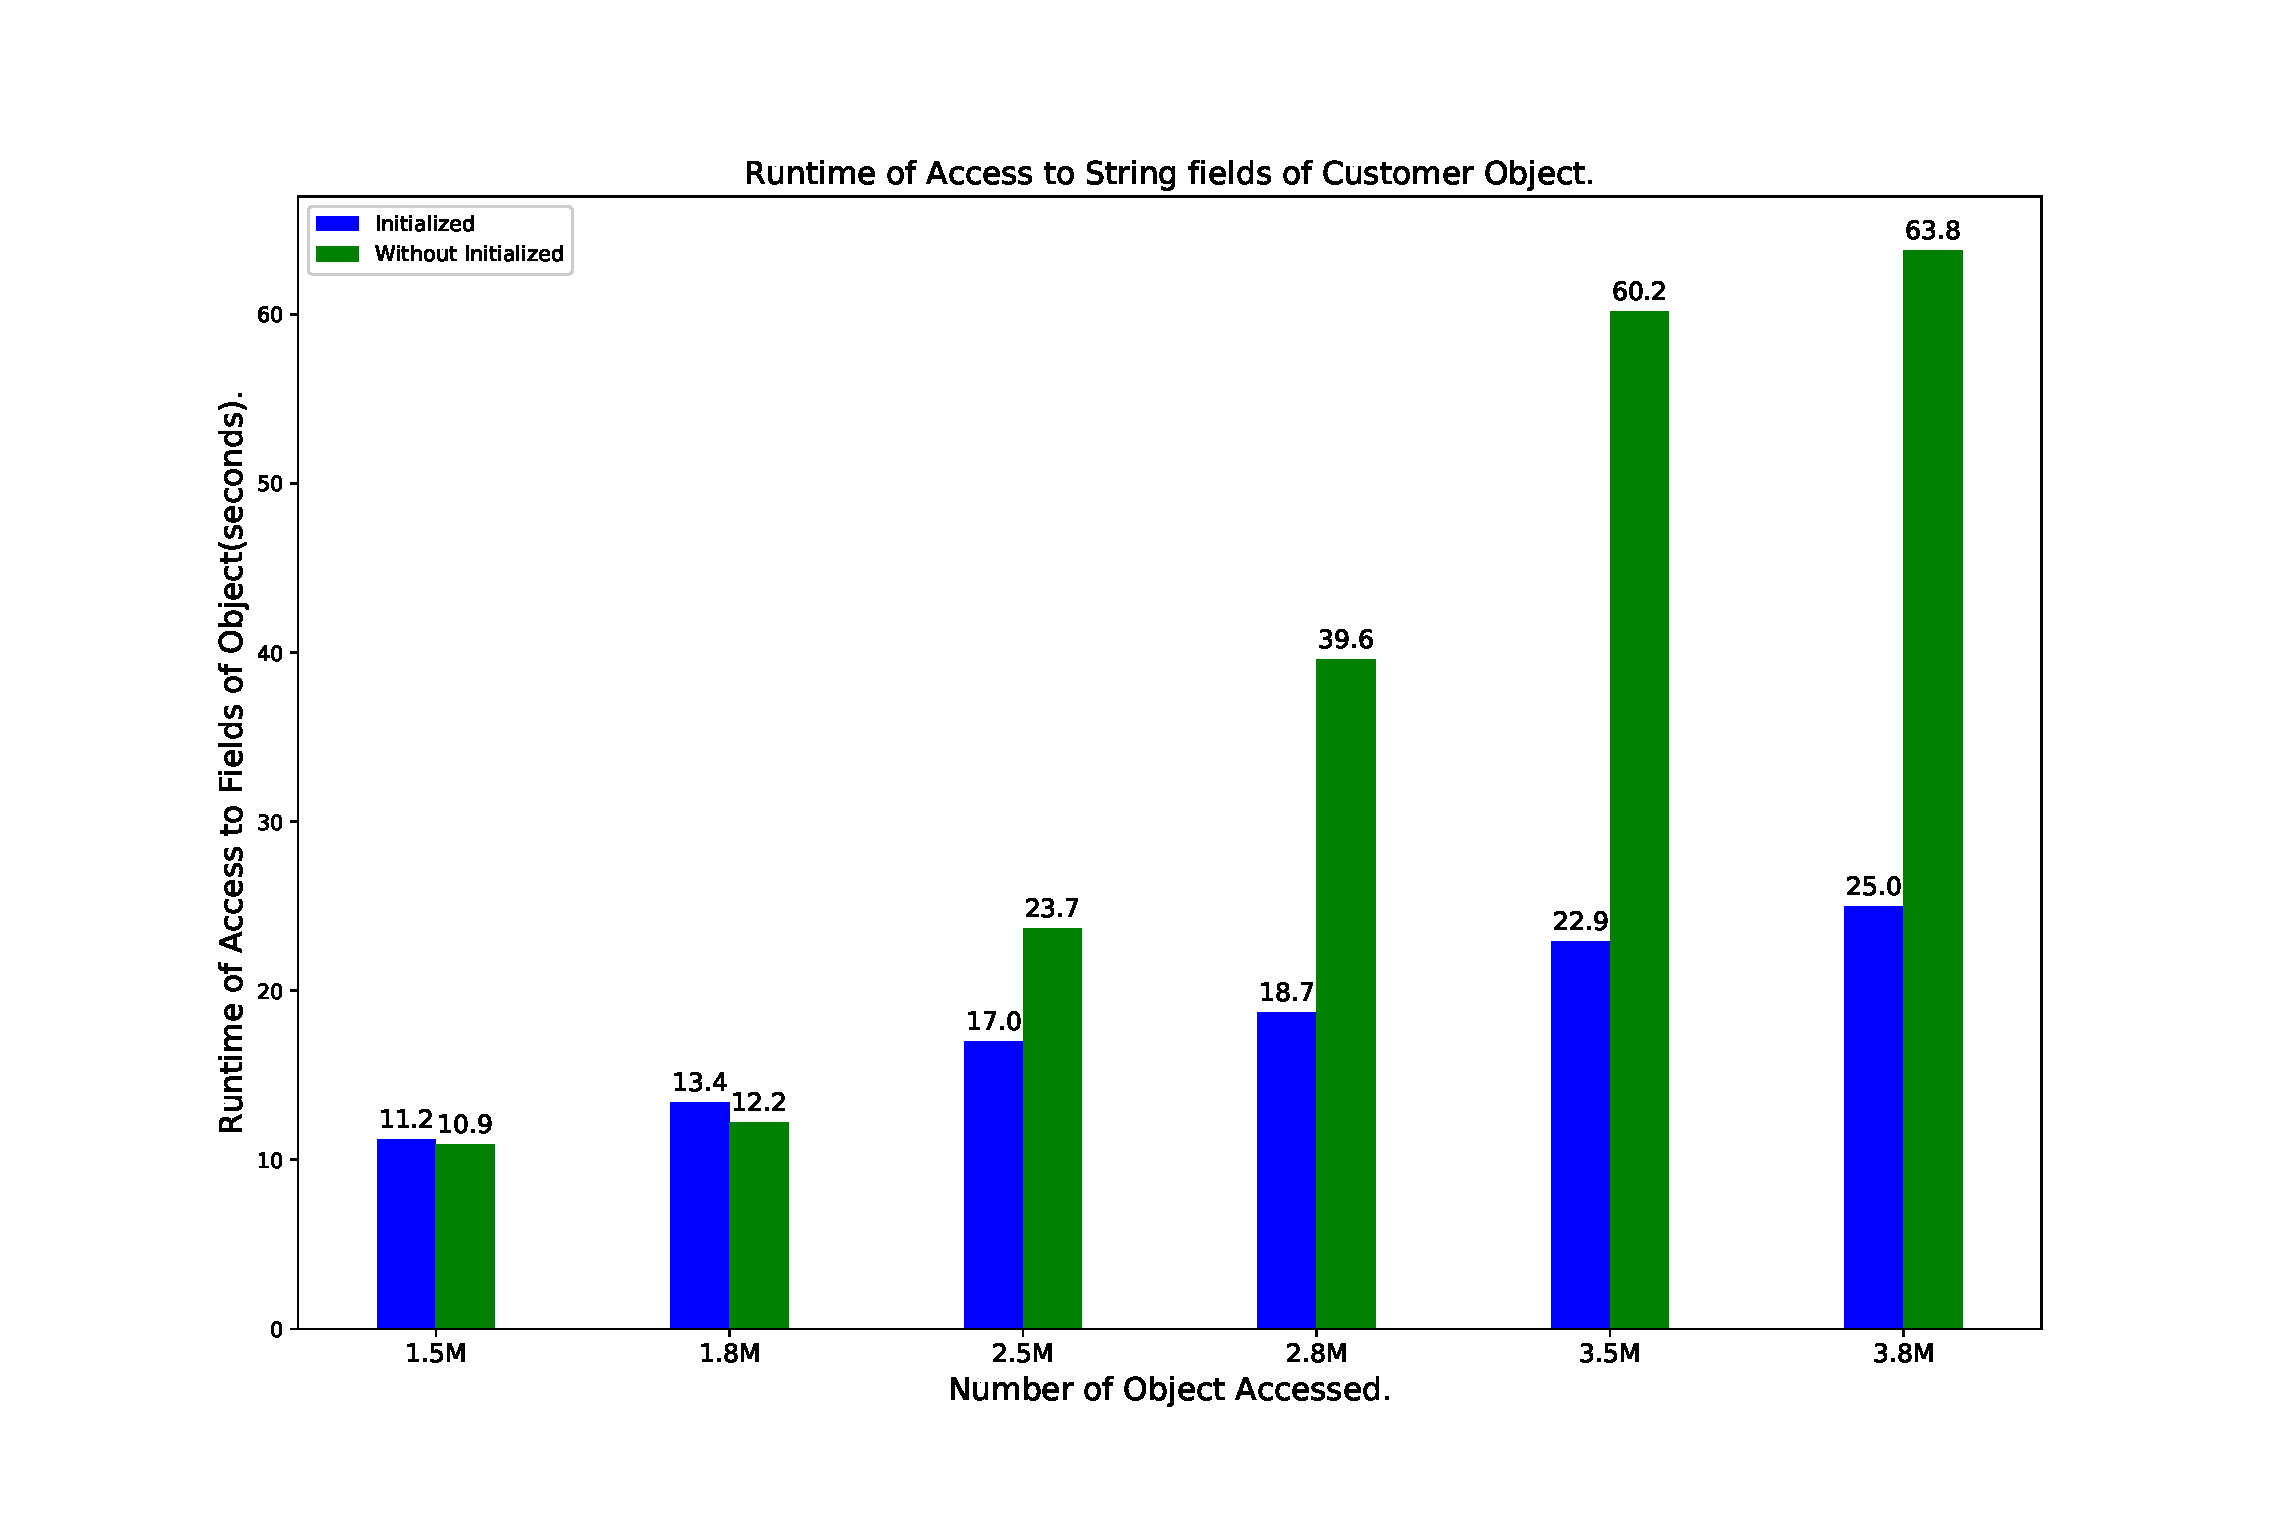
\includegraphics[width=15cm]{rust_access_init_vs_noint.eps}
    \caption{Runtime of Access to Fields of Complex Object with Initialization vs without Initialization}
    \label{fig:init_vs_noinit}
\end{figure}

\subsection{Discussion}
\label{sec:history}
Difference of variable types does not have huge impact to runtime of accessing to actual value.
Even thought owner, reference , and slice have different memory representations, the access time to its value is 
close to each other. As shown in Figure~\ref{fig:own_ref_slice}, the representations of owner and slice are almost identical except slice does not have capacity for values.
Reference is pointer pointing to owner, so it has an additional step to access actual value. 
However, the result shows this additional step does not have huge impact for runtime to access memory region of the value.

Whether initializing Vec size results in disparity of runtime performance to access objects' fields. 
This is because when Vec uninitialized, the elements of Vec are allocated across different virtual memory pages.

